\documentclass{beamer}

\usepackage{beamerthemesplit}
\usepackage[utf8]{inputenc}
\usepackage[ngerman]{babel}
\usepackage[justification=centering,figurename=Abb.]{caption}
\usepackage{pdfpages} 
\usepackage{listings} 
\usepackage{color}

\definecolor{dkgreen}{rgb}{0,0.6,0}
\definecolor{gray}{rgb}{0.5,0.5,0.5}
\definecolor{mauve}{rgb}{0.58,0,0.82}

\usetheme{Boadilla}
\useoutertheme[footline=authortitle]{miniframes}
\useinnertheme{rectangles}

\lstset{
    language=Java,
    tabsize=4,
    keepspaces,
    extendedchars=true,
    rulecolor=\color{black},
    keywordstyle=\color{blue},
    commentstyle=\color{dkgreen},
    stringstyle=\color{mauve},
    basicstyle=\footnotesize,
    aboveskip=5pt,
    upquote=true,
    columns=fixed,
    showstringspaces=false,
    extendedchars=true,
    breaklines=true,
    frame=single,
    showtabs=true,
    showspaces=false,
    showstringspaces=false,
}

\beamertemplatenavigationsymbolsempty

\begin{document}
\title{Einführungsvortrag: Entwurf einer GUI für den gMix-Simulator} 
\author[A. Beifuß, M. Weinschenk, J. Langnickel, J.Lohmüller]{Alexander Beifuß, Malte Weinschenk, Jörg Langnickel, Jan Carsten Lohmüller} 
\date{\today} 

\frame{\titlepage} 

\frame[t,squeeze]{\frametitle{Inhalt}
	\tableofcontents
}

\section{Motivation}

\frame[t,squeeze]{\frametitle{Motivation: Einführung in Mixe}
	Mixe wahren die Anonymität von Nutzern durch Bildung von Anonymitätsgruppen.
	\begin{columns}
		\begin{column}[t]{0.30\linewidth}
			\begin{itemize}
				\item Verschlüsselung
				\item Umkodierung
				\item Umsortierung
			\end{itemize}
		\end{column}
		\begin{column}[t]{0.68\linewidth}
			\begin{figure}
				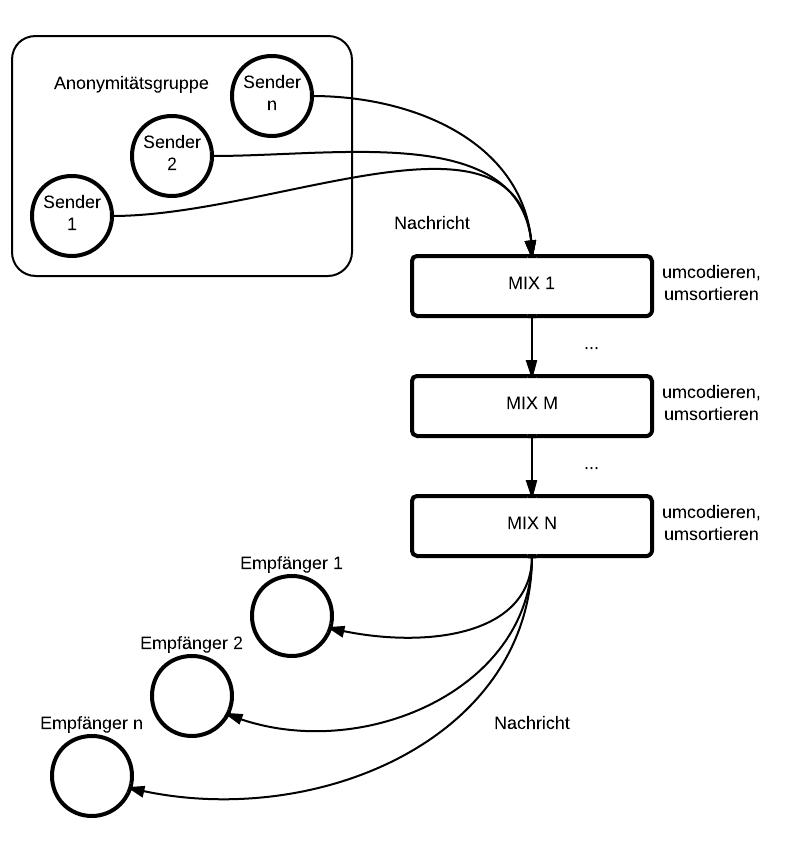
\includegraphics[scale=0.2, trim=0 0 0 15em]{konzeptmixeneu.png}
				\caption{Mixkaskade}
			\end{figure}
		\end{column}
	\end{columns}
}

\frame[t,squeeze]{\frametitle{Motivation: Bewertung von Mix-Systemen}
	Für die Forschungs- und Entwicklungsgemeinde ist es wichtige solche Systeme bewerten zu können.
	Ziele der Bewertung?
	\begin{itemize}
		\item Prototyping und Entwicklung von neuen Modellen
		\item Messung von Charakteristika (Bsp. Performanz, QOS-Parameter)
		\item Entwicklung von Verständnis für Mixe
	\end{itemize}
	Evaluationsmethoden:
		\begin{itemize}
			\item analytische Modelle (mathematischer Ansatz) \\
			\item Messung (Realsysteme) \\
			\item Simulation \\
		\end{itemize}
}

\section{Simulation}

\frame[t,squeeze]{\frametitle{Simulation: Gründe für Simulation}

	\begin{block}{Vorteile von Simulation}
		\begin{itemize}
			\item Skalierbarkeit
			\item Reproduzierbarkeit
		\end{itemize}
	\end{block}


	\begin{block}{Simulationen erlauben die einfache Parametrisierung bei Experimenten}
		\begin{itemize}
			\item Anzahl der Mixe
			\item Anzahl der Nutzer
			\item Ankunftsprozesse
			\item Bedienstrategien
			\item Flushing-Strategien
			\item ...
		\end{itemize}
	\end{block}
}

\frame[t,squeeze]{\frametitle{Simulation: (Netzwerk)Simulatoren}
	\begin{minipage}[t]{0.48\linewidth}
			\begin{itemize}
				\item ns2/ns3
				\item Opnet
				\item OMNet
				\item NetSim
				\item Large Scale Simulator
			\end{itemize}
			Problematik:
			\begin{itemize}
				\item Netzwerksimulatoren \\
				(keine Mix-Simulation)
				\item GUI teilweise nicht vorhanden
				\item Proprietäre Software
			\end{itemize}
	\end{minipage}	
	\begin{minipage}[t]{0.48\linewidth}
		\begin{figure}
			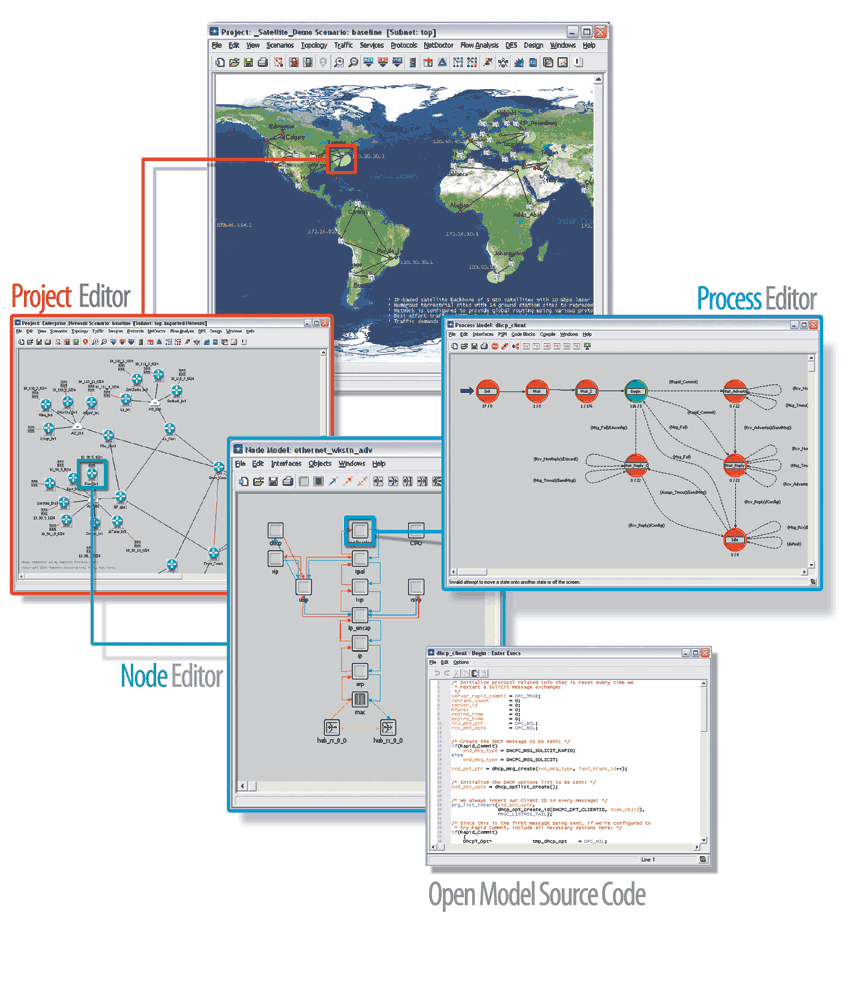
\includegraphics[scale=0.15]{opnet.png}
			\caption{Graphische modellierung mit Opnet Modeler}
				%Quelle: http://www.opnet.com/solutions/network_rd/images/OPNET-hierarchical-GUI-editors_lrg.gif
		\end{figure}
	\end{minipage}
}

\section{gMix}

\frame[t,squeeze]{\frametitle{gMix: Das Framework}

		... wurde speziell zur Simulation von Mixen entwickelt, wobei ein großer Wert auf die Erweiterbarkeit gelegt wurde.

		\begin{itemize}
			\item Last Generierung
				\begin{itemize}
					\item Bestimmung von Lastcharakteristika
					\item Modellierung der Clients
				\end{itemize}
			\item Simulation \& Messung
				\begin{itemize}
					\item Modellierung  der Mixe
					\item Konfiguration der Plug-Ins
				\end{itemize}
			\item Evaluation
				\begin{itemize}
					\item Auswertungs Plug-Ins
				\end{itemize}
		\end{itemize}

		Außerdem können mit Hilfe von gMix Mixe zu Messzwecken verteilt in richtigen Netzen aufgebaut werden.
}

\frame[t,squeeze]{\frametitle{gMix: Lastcharakteristika}

		\begin{block}{Vorgehensweise}
			\begin{enumerate}
				\item Host-Verhalten aus Verkehrsdaten extrahieren
				\item Host Datenbank erstellen
				\item Host selektieren
				\item Trace-File generieren
			\end{enumerate}
		\end{block}
		\begin{figure}
			\includegraphics[scale=0.97, page=9, trim= 4.70cm 25.6cm 4.0cm 10cm, clip=false]{../literatur/paper.pdf}
				%Quelle: https://svs.informatik.uni-hamburg.de/gmix/tutorialSimulator.php
		\end{figure}
}

\section[GUI]{Benutzbarkeit (GUI)}

\frame[t,squeeze]{\frametitle{GUI: Benutzbarkeit}
	\begin{block}{Aktuell}
		Es ist keine GUI vorhanden! \\
		$\Rightarrow$ Erschwerter Einstieg bei der Benutzung des Simulators
	\end{block}
	\begin{figure}
		\begin{minipage}[t]{0.48\linewidth}
			\vspace{0.3em}
			Zielgruppen für die GUI:
			\begin{enumerate}
				\item Nutzer in der Lehre
				\item Forscher
				\item Entwickler von Plugins
			\end{enumerate}
		\end{minipage}
		\begin{minipage}[t]{0.48\linewidth}
			\centering
			\begin{figure}
				\includegraphics[scale=0.2, page=6]{../mockup/myBalsamiqProject.pdf}
				%Quelle: https://svs.informatik.uni-hamburg.de/gmix/tutorialSimulator.php
			\end{figure}
		\end{minipage}
	\end{figure}
}

\section{Ausgangssituation}
\frame[t,squeeze]{\frametitle{Ausgangssituation: Die Konfigurationsdateien}

	\begin{block}{Zentrale Konfigurationsdatei(n)}
		\begin{itemize}
			\item simulatorConfig.txt
			\item experimentDefinitions/...
		\end{itemize}
	\end{block}

	Die Experiment-Definition wird je Experiment eingelesen.\\
	Der Zugriff erfolgt mittels 'Settings.getProperty(String key)'.

	\begin{block}{Plugin spezifische Konfigurationsdatei (gMixGui, Marius Fink)}
		PlugInSettings.txt
	\end{block}

	Das Tool 'gMixGui' könnte Teilweise wiederverwendet werden, da es Überschneidungen mit der von uns zu entwickelnden Software / GUI aufweist.
}

\section{Technologien}
\frame[t,squeeze]{\frametitle{Technologien: XML vs. Annotations}
	\begin{block}{statische Ansätze}
		\begin{itemize}
			\item statische GUI
			\item globale XML global
		\end{itemize}
	\end{block}
	\begin{block}{dynamische Ansätze}
		\begin{itemize}
			\item XML je plugin (gMixGui)
				\begin{itemize}
					\item zentral
				\end{itemize}
			\item Annotations
				\begin{itemize}
					\item Direkt im Source-Code
					\item Kein aufwändiges Parsen von XML notwendig
					\item Einfach anpassbar / erweiterbar
				\end{itemize}
		\end{itemize}
	\end{block}
}

\begin{frame}[fragile]{Technologien: Annotations Beispiel}
\lstset{language=Java}
\begin{lstlisting}[caption={Beispiel zur Anwendung von Annotations}]
public class MixPlugIn extends Implementation implements Layer3OutputStrategyMix {

    private SimplexBatch requestBatch;
    private SimplexBatch replyBatch;
    
    @SimulationProperty(name = "Batch size", 
        description = "The batch size is ... <some text>", 
        tooltip = "Size of the batch",
        minValue = 0, 
        maxValue = 255, 
        category = "Mix Strategy")
    private int BATCH_SIZE;
    ...
}
\end{lstlisting}
\end{frame}

\frame[t,squeeze]{\frametitle{Technologien: Beispiel eines Abhängigkeitsgraphen}
	\begin{figure}
	    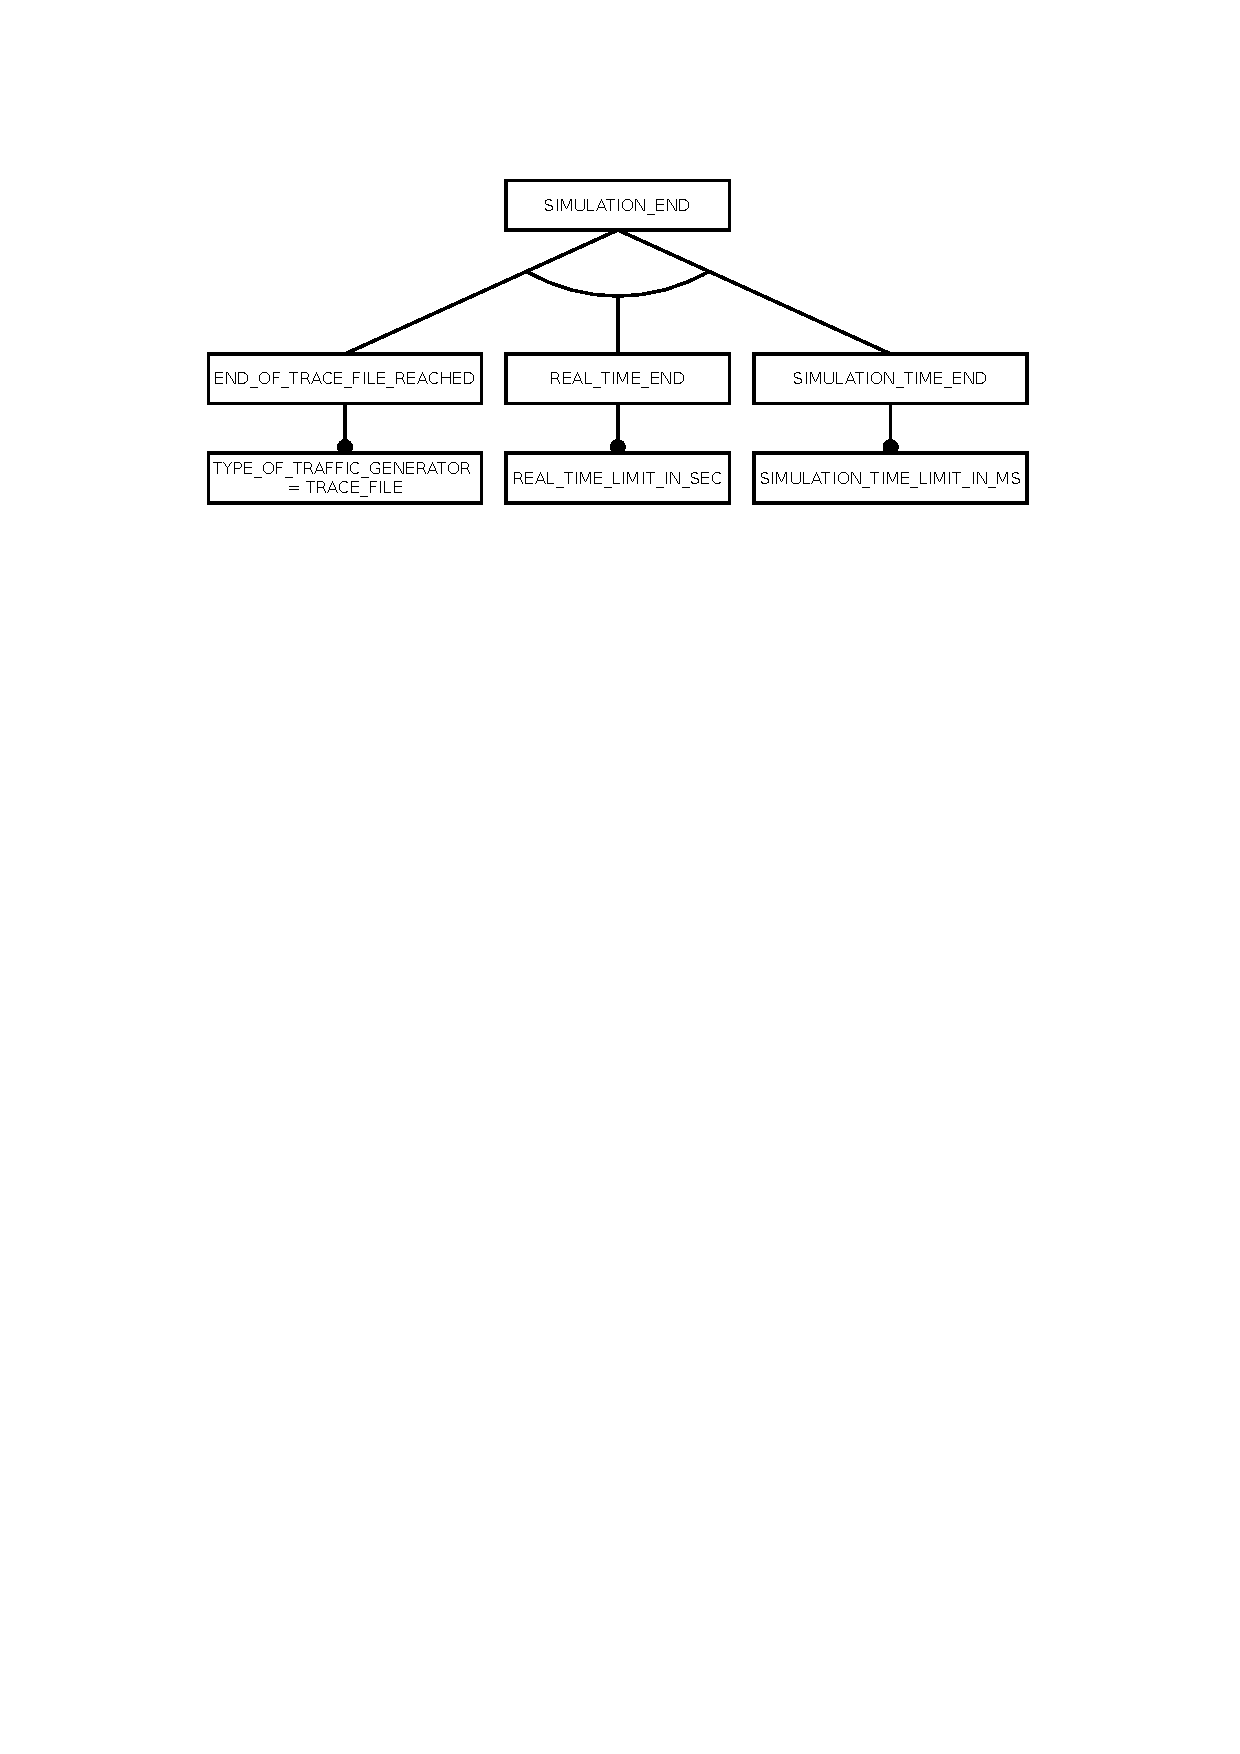
\includegraphics[scale=0.85, trim=5cm 0cm 5cm 2.5cm]{featuremodel.pdf}
	\end{figure}
}

\section{Mock-Ups}
\frame[t,squeeze]{\frametitle{Mock-Ups: Ziele für die GUI}
	\begin{itemize}
		\item übersichtliche / intuitive GUI
			\begin{itemize}
				\item Platzausnutzung (Smart Phone Elemente)
				\item Shortcuts / mehrere Wege
			\end{itemize}
		\item sinnvolle Strukturierung der Konfiguration
			\begin{itemize}
				\item liegt bereits vor... (Experiment Konfigurations Datei)
			\end{itemize}
		\item Bereitstellung von Automatisierungen / Unterstützungen
			\begin{itemize}
				\item Tool Tips
				\item Hilfe-System
				\item Abhängigkeiten auflösen
			\end{itemize}
	\end{itemize}
}

\frame[t,squeeze]{\frametitle{Mock-Up: Home View}
	\begin{figure}
	    \includegraphics[scale=0.37, page=6]{../mockup/myBalsamiqProject.pdf}
	\end{figure}
}

\frame[t,squeeze]{\frametitle{Mock-Up: (Video)Tutorial View}
	\begin{figure}
	    \includegraphics[scale=0.37, page=4]{../mockup/myBalsamiqProject.pdf}
	\end{figure}
}

\frame[t,squeeze]{\frametitle{Mock-Up: Simulator View}
	\begin{figure}
	    \includegraphics[scale=0.37, page=1]{../mockup/myBalsamiqProject.pdf}
	\end{figure}
}

\frame[t,squeeze]{\frametitle{Mock-Up: Results View}
	\begin{figure}
	    \includegraphics[scale=0.37, page=2]{../mockup/myBalsamiqProject.pdf}
	\end{figure}
}

\frame[t,squeeze]{\frametitle{Mock-Up: Console View }
	\begin{figure}
	    \includegraphics[scale=0.37, page=3]{../mockup/myBalsamiqProject.pdf}
	\end{figure}
}

\frame[t,squeeze]{\frametitle{Mock-Up: Help View}
	\begin{figure}
	    \includegraphics[scale=0.37, page=5]{../mockup/myBalsamiqProject.pdf}
	\end{figure}
}

%\begin{frame}[allowframebreaks]
%\frametitle{Quellen}
%\nocite{*}
%\printbibliography
%\end{frame}

\section{Diskussion}
\frame{
\begin{center}
	\huge{Diskussion}
\end{center}
}


\end{document}
